\section{Tests}
\subsection{Unit Tests}

\subsection{Hydro Tests}
\subsection{Linear Wave}
Sound waves provide the mechanism to transport disturbances in a fluid. An
elementary test problem is the ability maintain wave propagation of small
disturbances . Given a fluid in equilibrium with constant density $\rho_0$,
pressure $p_0$ and zero velocity $\mathbf{v}=0$ with perturbations of the form
\begin{equation}
	\begin{array}{rcl}
		\rho & = & \rho_0 + \delta\rho(x,t) \\
   		 p & = & p_0 + \delta p(x,t) \\
    	\mathbf{v} & = & \delta\mathbf{v}(x,t),
    \end{array}
\end{equation}
and maintaining terms to first order in the Euler equations produce the wave
equation for each variable with a wave propagation speed equal to the fluids sound speed 
$c_s$ suffice the perturbations are small. Thus, setting a small disturbance will propagate 
with a finite velocity maintaining 
its form.

We set up a 2d box of unit length with constant $\rho_0=1.0$, $p_0=3/5$, $\mathbf{v}=0$,
and $\gamma=5/3$ with periodic boundary conditions. A sinusoidal wave in the x direction of 
the form $\delta\rho(x,t) = Asin(kx + wt)$ with $k=w=2\pi$ and $A=10^{-6}$ is added at time 
$t=0$. The remaining disturbances can be specified through $\delta\rho$ by the following
\begin{equation}
	\begin{array}{rcl}
        \delta \mathbf{v}(x,0) & = & \left(\frac{w}{k}\right)\delta
        	\rho(x,0)/\rho_0\mathbf{\hat{x}}\\
        \delta p(x,0) & = & \left(\frac{w}{k}\right)^2\delta\rho(x,0).
    \end{array}
\end{equation}
The values chosen produce waves traveling rightward with a velocity of 1. The simulation is
ran for 1 time unit such that the waves return to its initial position at time $t=0$. 
Moreover, we study the convergence behavior by comparing the final state of the density to 
the initial density by computing the $L1$ norm,
\begin{equation}
	L1 = \frac{1}{N^2}\sum_i \left| \rho_i - \rho(x_i) \right|,
\end{equation}
where $\rho_i$ is final density at position $x_i$ and $\rho(x_i)$ is the density at t=0
at position $x_i$ and $N$ is the number of cells per dimension. Five simulations where ran
with varying resolution $N=10, 20, 40, 80, 160$. The initial particles where laid out in a
Cartesian grid and the mesh was allowed to move with the fluid velocity. All simulations
where performed with linear reconstruction and the HLLC solver.
\begin{figure}
    \begin{center}
        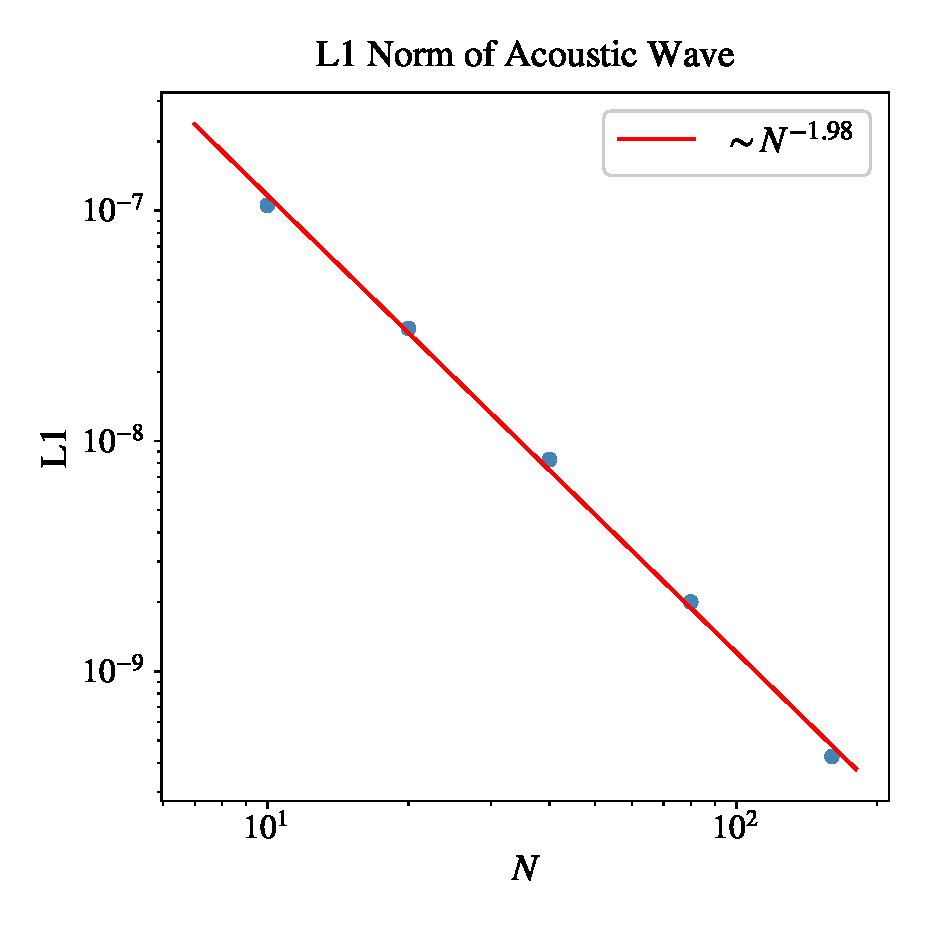
\includegraphics[width=0.4\textwidth]{figures/acoustic-wave-l1.eps}
        \caption{L1 norm of acoustic wave problem in 2d. Blue points are results
        of simulation from different resolutions overlayed by a linear fit showing
        the convergence is approximately second order.}
        \label{fig.acoustic}
    \end{center}
\end{figure}


\subsubsection{Sod Shock Tube}
\subsubsection{Sedov}
\subsubsection{Kelvin Helmholtz}

\subsection{Gravity Tests}
\subsubsection{Rayleigh Taylor}
\subsubsection{Two body}
\subsubsection{Evrard Collapse}

\subsection{Chemistry Tests}
\subsubsection{Uniform Cooling}
